\documentclass[11pt, oneside]{article}   	% use "amsart" instead of "article" for AMSLaTeX format
\usepackage{geometry}                		% See geometry.pdf to learn the layout options. There are lots.
\geometry{letterpaper}                   		% ... or a4paper or a5paper or ... 
%\geometry{landscape}                		% Activate for rotated page geometry
\usepackage[parfill]{parskip}    		% Activate to begin paragraphs with an empty line rather than an indent
\usepackage{graphicx}				% Use pdf, png, jpg, or eps§ with pdflatex; use eps in DVI mode
								% TeX will automatically convert eps --> pdf in pdflatex		
\usepackage{amssymb}
\usepackage{achemso}
\usepackage{graphicx}
\usepackage{url}

%SetFonts

%SetFonts


\title{Converging Interests- Chemoinformatics, History, and Bibliometrics}
\author{Wenxi Zhao, Dmitriy Korobskiy, Shreya Chandrasekharan, \\Kenneth Merz, George Chacko}
%\date{}							% Activate to display a given date or no date

\begin{document}
\maketitle
%\section{}
%\subsection{}

In this Viewpoint, we briefly discuss using citation analysis for historical insight into a scientific field. We emphasize that citations can tell only a part of the story but are still valuable in tracing historical developments in a field, and the consideration of new ideas within it. We use the the quantum mechanical (QM) density functional theory (DFT) model referred to as B3LYP, where B3 refers to the Becke 3-parameter Exchange functional and LYP to the Lee, Yang and Parr Correlation functional.

 The chemoinformatics literature has previously been analyzed by Willett~\citep{willett2008}, who has also written about the history of chemoinformatics\citep{willett2003}, who comments that  `Chemoinformatics first appeared as a distinct discipline in the late-Nineties, since when it has generated a considerable literature'. Willett cites preceding studies by Onodera~\citep{onodera2001,onodera2003} on chemical informatics using bibliographic data. Willett also cites methods from scientometrics~\citep{garfield2004,leydesdorff2007}.  Of the two scientometric methods cited by Willett, algorithmic historiography~\citep{garfield2004} merits special mention since it involves constructing a historical record using scientific citations. The chemoinformatics community has thus experienced intersections with science history and bibliometrics (the terms bibliometrics, scientometrics, and informetrics have been interchangeably used to refer to quantitative studies of the scientific literature~\citep{debellis2009}).
 
More recently Williams and colleagues (2015)\citep{williams2015scientific} have used the principles of algorithmic historiography coupled with data mining and network analysis to describe the very large collaboration networks that contributed to the basic and translational work preceding the development of two breakthrough drugs. We\citep{keserci2017research} have further built upon the work of Williams to analyze, at greater scale, similar networks for five anti-cancer drugs also approved for human use by the Food and Drug Administration (FDA), a study that involved analyzing the work of 235,000 authors of 106,000 publications.

Modern bibliographic databases such as Scopus and Web of Science greatly assist such studies since their coverage is extensive and their content (available through a commercial license) can be incorporated into relational or graph databases for large scale analysis. Citation data are neither complete nor error free~\citep{macroberts2017} but are still immensely useful, and the data available today are improved over what was available decades ago. 

Three major patterns of citation have been described: (i) direct citation (ii) bibliographic coupling and (iii) co-citation. When an article cites or references another article a direct citation link is created between the citing article and its target, the cited article. Many such links to a cited article causes it to accumulate citations, which are sometimes used to estimate its impact. When two articles cite a third, they are bibliographically coupled~\citep{Kessler1963}. When two articles are cited by a third, they are said to be co-cited with the implication that two previously existing ideas are combined into a new one. Co-citation was independently described by Marshakova-Shaikevich and Small in 1973~\citep{MarshakovaShaikevich1973,Small1973} and co-citation measurements have since been extensively used in scientometrics. The frequency of co-citation of a pair of articles  also accumulates over time and represents the extent to which this new idea is recognized by the research community. In this respect, co-citation is a dynamic measure compared to bibliographic coupling. The vast majority of articles are cited or co-cited once or not at all. Thus, highly cited or co-cited articles naturally pique interest. 


From a sampling of the physics literature, Small~\citep{Small1973} in 1973, reported 4 pairs of articles with a co-citation frequency of 49 and greater. The volume of scientific literature has since grown considerably; more co-cited pairs have been discovered, citation frequencies have increased, and the scale of bibliometric studies has also increased. Improved bibliographies and modern computing tools have also rendered co-citation calculations relatively facile and co-citation has been measured over tens of millions of articles, and the high end of co-citation frequencies is in the tens of thousands~\citep{Stringer2010,Uzzi2013,devarakonda_2020}. Interestingly, in a large scale study of co-citation patterns across the all scientific literature~\citep{devarakonda_2020}, the articles by (i) Becke (1993)\citep{becke1993dft} and (ii) Lee, Yang, and Parr (1988)\citep{lyp1988} were the most highly co-cited pair of 33 million such pairs that we studied. In extension of this study~\citep{devarakonda_2020}, we present below, an analysis that is centered around these two articles. 

A natural extension of co-citation theory is document coupling of a higher order, for example, triads and tetrads that are correspondingly tri-cited and tetra-cited. It is possible to view any article $A$ that cites $n$ articles as comprising $n$ citations, $n\choose2$ co-citations, $n\choose3$ tri-citations and so on. Indeed, Henry Small proposed a model of multiple citation in 1974~\citep{small1974multiple} based on tri-citations measured over a set of 6 publications.  Calculating the frequencies of these combinations in a bibliography is relatively expensive, however, and may have dissuaded follow-up investigations. For example, an article with either 25 or 50 cited references represents 300 or 1,225 co-citations respectively. The same article also consists of  2,300 or 19,600 tri-citations and  12,650 or  230,300 tetra-citations. For even a modestly sized collection of 2 million articles with an average of 30 references each, this could involve computing $8.12\times10^9$ tri-citations, $5.48\times10^{10}$ tetra-citations, or $2.85\times10^{11}$ penta-citations. However, today's computing resources place documenting these higher order structures within reach of the scientometrist, and opens a frontier for discovery that extends beyond co-citation.



In an initial exploration of higher-order combinations, we have used a `brute force' approach to compute the tri-citation frequencies of 181 million triads from 11 years of articles in the Scopus bibliography.  Much like citations and co-citations, the vast majority of tri-citations are of very low frequency, suggesting modest community recognition. High frequency triplets are therefore, of interest. The triad with the highest frequency that we observed in 181 million cases has been tri-cited at least 13,000 times and all three of its component articles derive from density functional theory (DFT). 
\begin{figure}[h!]
\begin{center}
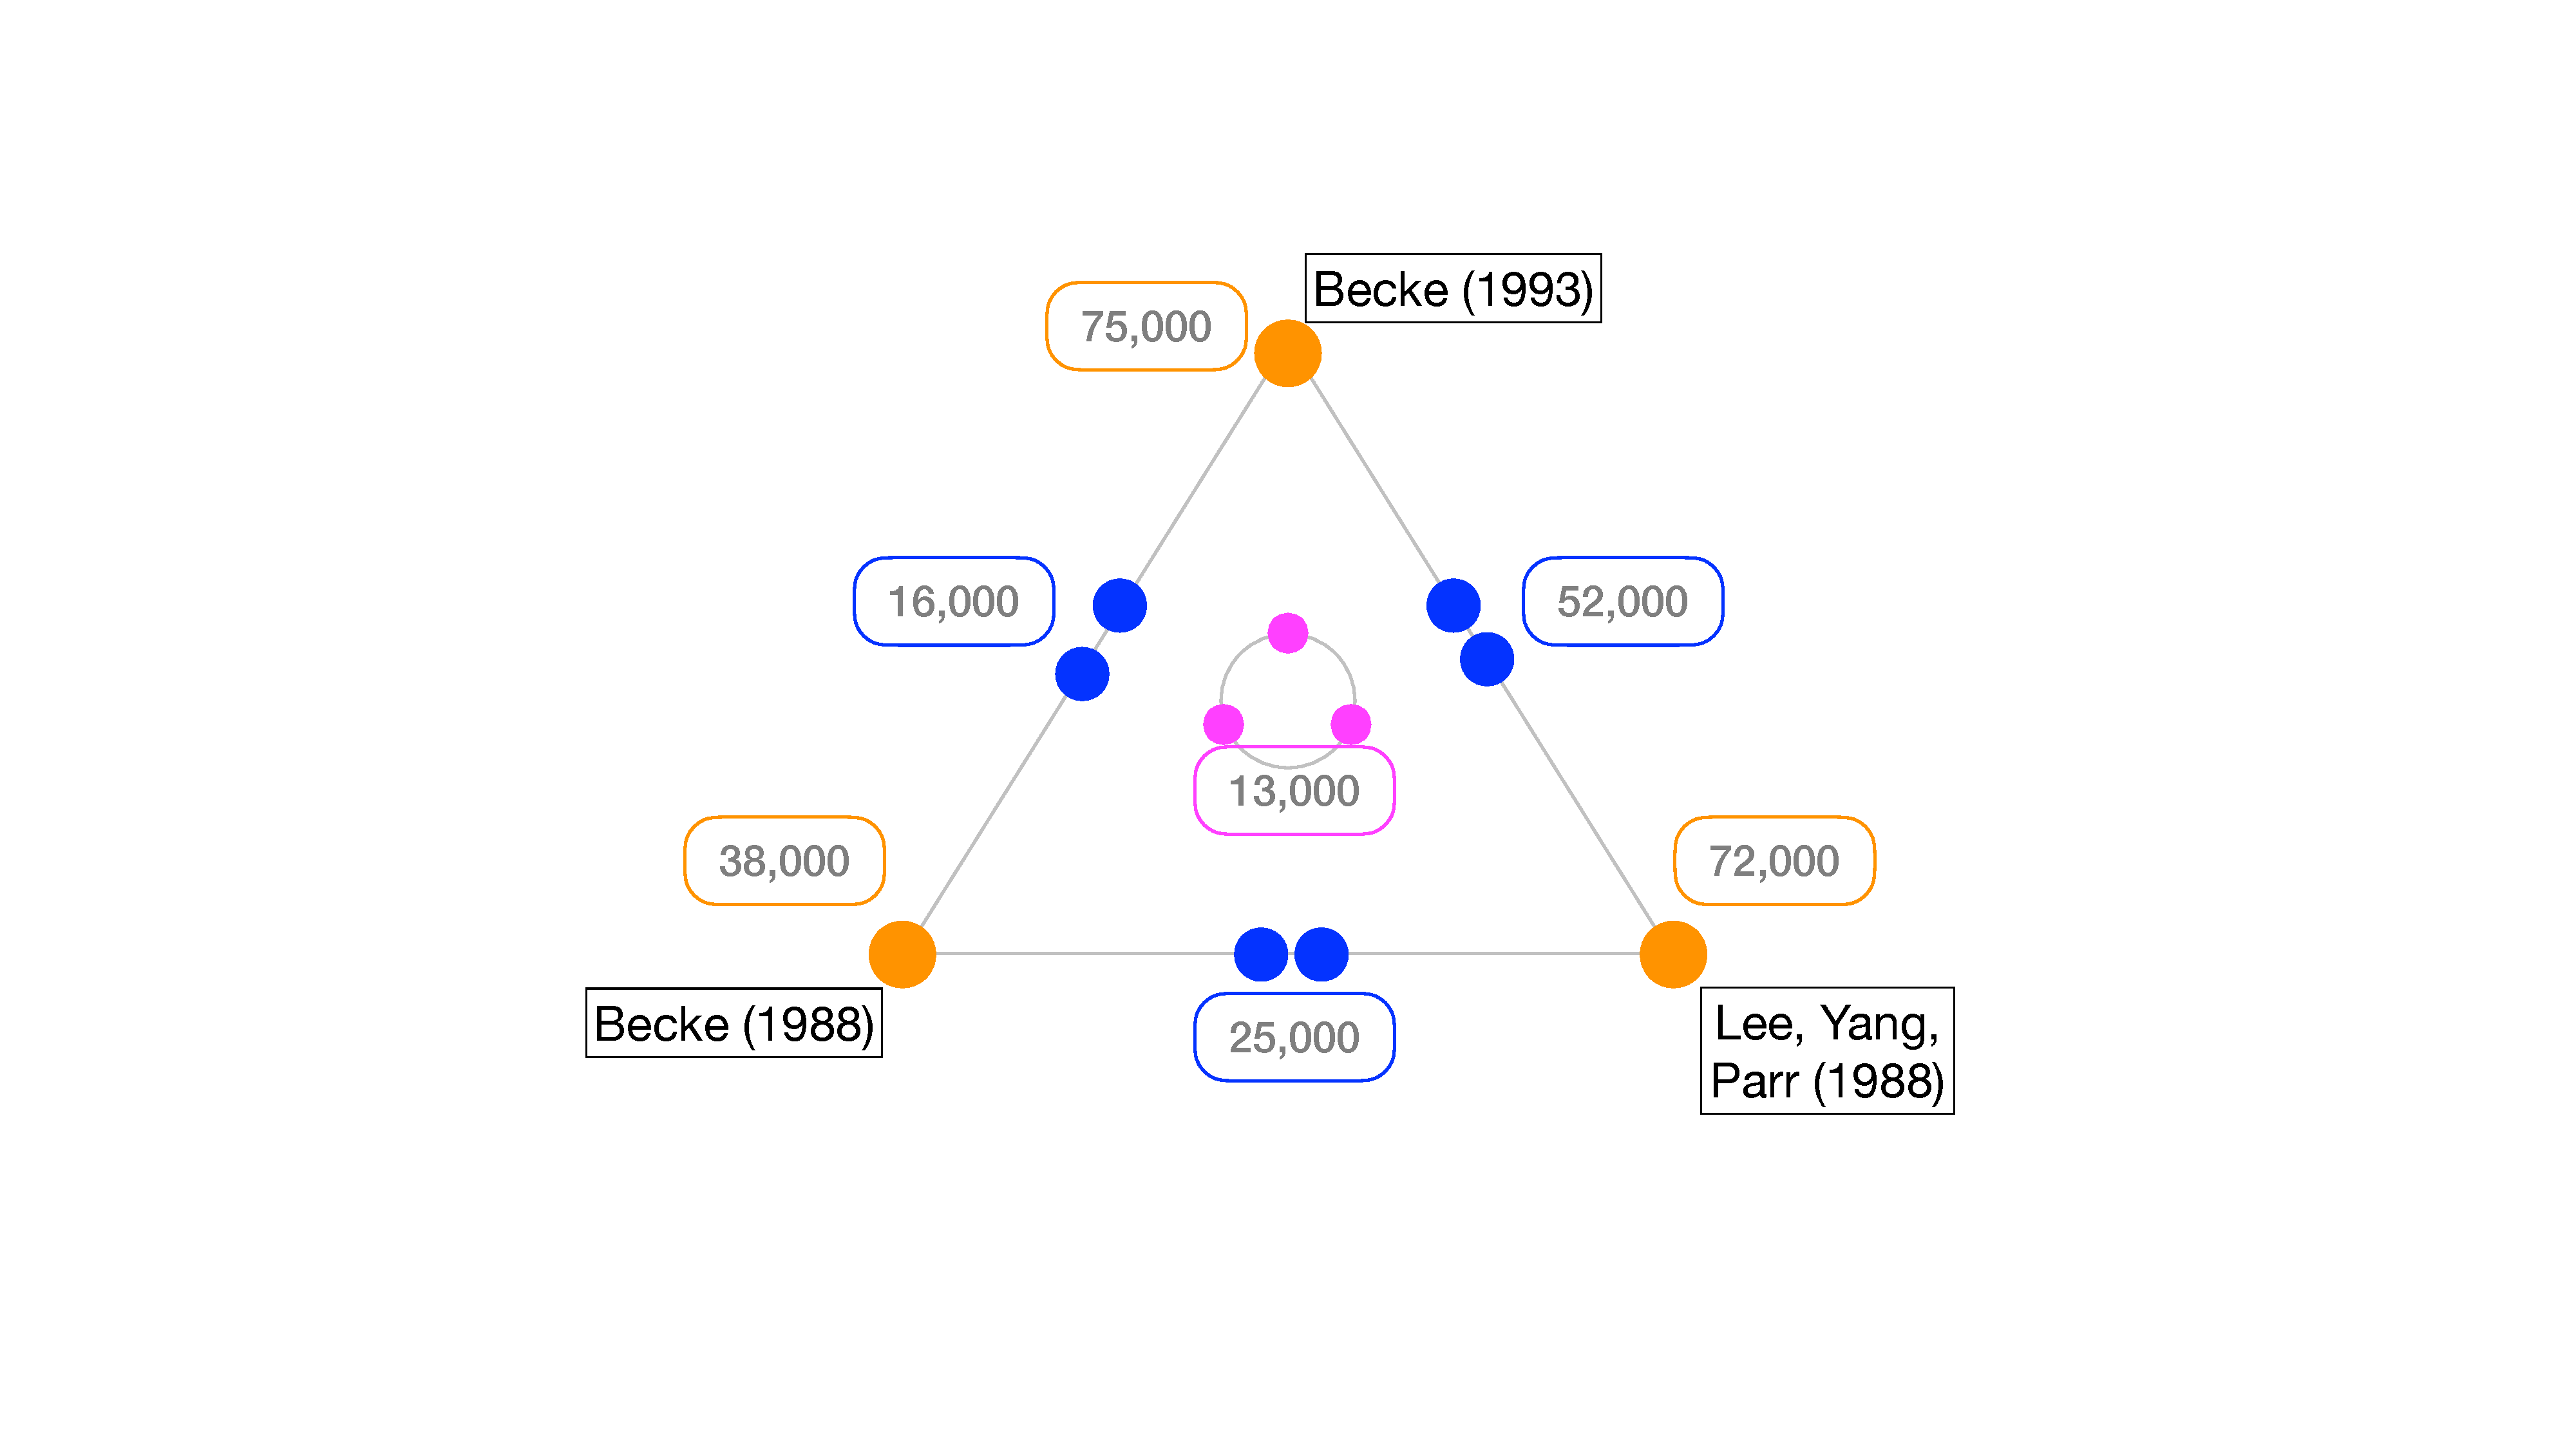
\includegraphics[width=10cm]{fig1_tricite.pdf}% This is a *.eps file
\end{center}
\caption{A high frequency triplet. The triad of (i) Becke (1988), (ii) Becke (1993), and (iii) Lee, Yang, and Parr (1988).  Frequencies (rounded rectangles) are shown for the tri-citation (center of triangle), co-citations (sides of triangle), and article citations (vertices of triangle). All frequencies shown have been rounded down to the nearest thousand
}
\label{fig:fig1}
\end{figure}

The origin of this triad appears to trace back to 1994, when Stephens, Chabalowski, Devlin, and Frisch~\citep{stephens1994ab} blended the B3 Exchange and LYP Correlation functionals into a hybrid functional method currently  referred to as B3LYP.  The first referencing of this triad appears to be in two reports in 1993: (i) an article by Laming, Temath, and Handy\citep{laming1993} titled `A general purpose exchange‐correlation energy functional' and (ii) a chapter titled `Theoretical Organic Chemistry' in Annual Reports Section ``B" (Organic Chemistry) by Reynolds\citep{reynolds1993theoretical}.

In the B3LYP model, two functionals of the electron density are needed. One is the Exchange functional (two electrons of the same spin cannot be at the same point in space) and the other is the Correlation functional (accounting for the correlated motion of electrons with the same spin). The B3LYP method had a lot of advantages in terms of speed and accuracy, especially for the study of organic molecules, and was rapidly adopted by the computational chemistry and organic chemistry communities. Historically, B3LYP originates from an effort in the 1980s to to build Exchange and Correlation functionals to allow for the practical application of DFT to chemical problems. A number of research groups engaged and the Becke group in 1988 and 1993 described a hybrid functional~\citep{becke1988density}, and an Exchange functional~\citep{becke1993dft}, respectively, while Lee, Yang, and Parr (LYP) developed a Correlation functional in their 1988 paper~\citep{lyp1988}.  

This major advance can be concisely referenced by citing Becke-1988~\citep{becke1988density}, LYP-1988~\citep{lyp1988} and Becke-1993~\citep{becke1993dft} since the two Becke articles represent the Exchange functional and the Lee-Yang-Parr article contributes the Correlation functional. The high frequency of co-citation (52,000) of Becke-1993 and LYP-1988 may result from authors assuming or concluding that citing Becke's 1993 article is adequate to reference the Exchange functional. 

Based on our use of Scopus data, the three articles in the Becke-1988--LYP-1988--Becke-1993 triad appear to have been co-cited at least 16,000, 25,000, and 52,000 times respectively, and the individual articles cited at least 38,000, 72,000, and 75,000 times (Figure 1). It is more difficult to conjecture why these three articles are individually cited at these very high levels although it is worth noting that  frequencies of article citations always exceed those of co-citations, which in turn exceed those of tri-citations. It is also very likely that these articles have individually stimulated new ideas.

An interesting community discussion thread~\citep{johansson2002} provides the opinion that a complete set of citations for B3LYP is (i) Vosko, Wilk and Nusair, 1980~\citep{vosko1980accurate} or VWN-1980 (ii) Becke-1988) (iii) LYP-1988) (iv) Becke-1993) and (v) Stephens, Chabalowski, Devlin, and Frisch (1994) or SCDF-1994. It is interesting to note that VWN-1980  is not cited in Becke (1988), Becke (1993), or LYP (1993) although it is cited in Laming et al. (1993), Reynolds (1993), and SCDF-1994.

In this demonstration of the use of citation data, we describe a high frequency triad discovered through a discipline-agnostic search that led us to a cluster of publications that are associated with a major advance in  in the practical application of DFT to chemical and biological problems. Examining the three component co-cited pairs of the triad allows us to infer that Becke (1993) and LYP (1988) are most extensively recognized in the community as far as B3LYP is concerned. Why Becke-1988 is not more often co-cited with Becke (1993) and LYP (1988) is an interesting question along with why VWN (1980) is not generally included with these three papers forming a highly cited cluster of four papers. The same question can be asked regarding SCDF (1994) which merged the technologies of these these four publications into what is now known as the B3LYP Exchange-Correlation function.  Inferring or understanding the social behavior in the community that resulted in these citation patterns will require further qualitative research. In the meantime, it may be reasonable to conclude that B3LYP has had high impact in chemoinformatics and generates curiosity in the scientometrics world.

\bibliographystyle{acm}
\bibliography{B3LYP}

\end{document}  